\documentclass[../../numcalc]{subfiles}

\begin{document}
\chapter{数値微分}
\label{chapter:numerical_differentiation}
\begin{lead}
数値微分は,微分係数を近似計算する手法である.
微分方程式や最適化問題の数値解を求めるとき,数値微分は非常に重要な役割を持つ.
\cref{chapter:numerical_differentiation}では,補間多項式を利用して数値微分の一般式を導き,その性質を調べていく.
\end{lead}

\section{数値微分}
関数を補間多項式で近似できるのなら,関数の微分係数もまた,補間多項式の微分係数で近似できると考えられる.
すなわち,\(t\)の値が標本点\(x_1,\dots,x_n\)の値に十分近いとき,点\((x_1,f(x_1)),\dots,(x_n,f(x_n))\)に関する補間多項式を\(p_n(x)\)とすると\(f'(t)\fallingdotseq\eval{p_n'(x)}_{x=t}\)であると期待できる.

このような微分の近似を\impact{数値微分}\index{すうちびぶん@数値微分}(numerical differentiation)という.数値微分をするときは\(x_1,\dots,x_n\)を等間隔に取ることが多い.以下にこの場合の例を示す.

\begin{example}
\label{example:numerical_derivative_1}
\((x_1,x_2)=(t,t+h)\)のとき\(p_2(x)=f(t)+\divdiff[f]{t,t+h}(x-t)\)である.よって,\(p_2(x)\)に基づく\(f\)の数値微分は
\[
  f'(t) \fallingdotseq \eval{p_2'(x)}_{x=t}
  = \divdiff[f]{t,t+h}
  = \frac{f(t+h)-f(t)}{h}
\]
となる.\(h\to 0\)では,右辺は厳密に\(f'(t)\)と等しくなる.
\end{example}

\begin{example}
\label{example:numerical_derivative_2}
\((x_1,x_2,x_3)=(t-h,t,t+h)\)のとき
\[
  p_3(x) = f(t-h)+\divdiff[f]{t-h,t}\pqty*{x-(t-h)}+\divdiff[f]{t-h,t,t+h}\pqty*{x-(t-h)}(x-t)
\]
である.よって,\(p_3(x)\)に基づく\(f\)の数値微分は
\begin{align*}
  f'(t) &\fallingdotseq \eval{p_3'(x)}_{x=t} = \divdiff[f]{t-h,t}+\divdiff[f]{t-h,t,t+h}h \\
  &= \frac{f(t)-f(t-h)}{h}+\frac{(f(t)-f(t-h))/h-(f(t+h)-f(t))/h}{(t-h)-(t+h)}h \\
  &= \frac{f(t+h)-f(t-h)}{2h}  
\end{align*}
となる.この式についても,\(h\to 0\)では
\[
  \frac{f(t+h)-f(t-h)}{2h} = \frac{f(t+h)-f(t)}{2h}+\frac{f(t)-f(t-h)}{2h}
  \to f'(t)\quad(h\to 0)
\]
が成立する.
\end{example}

\begin{figure}[htbp]
  \centering
  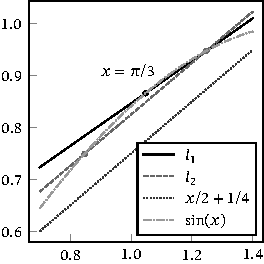
\includegraphics{differentiation.pdf}
  \caption{数値微分の比較}
  \label{figure:differentiation}
\end{figure}

\cref{figure:differentiation}は,2つの直線
\begin{align*}
  l_1 &\colon y=\frac{f(t+h)-f(t)}{h}(x-t)+f(t), \\
  l_2 &\colon y=\frac{f(t+h)-f(t-h)}{2h}(x-(t-h))+f(t-h)
\end{align*}
を\(f(x)=\sin(x)\),\(t=\krez/3\),\(h=0.2\)の場合について示したものである.
\cref{figure:differentiation}によれば,\(l_2\)は\(l_1\)よりも傾きが\(1/2=\cos(\krez/3)\)に近い.
したがって,\((\sin(x))'\)の\(x=\krez/3\)における近似に関しては,\cref{example:numerical_derivative_1}よりも\cref{example:numerical_derivative_2}のほうが真値に近い値を与えている.
より一般に,\(h\)の値を変えない場合,高次の補間多項式を利用した公式ほど近似値は真値に近づく傾向にある.

\end{document}
